\section{Experimentation}
\label{sec:experimentation}

Semi-autonomous systems explore efficient policy execution involving the optimal transfer of control between human and agent~\cite{Cohn11-SemiAutonomousAgents}. Our focus is on semi-autonomous driving, namely the optimal policy to adapt to a human's level of fatigue.

The LMDP consists of states formed by a 4-tuple: current intersection, previous intersection, driver tired (true/false), and autonomy (enabled/disabled). Actions are taken at intersections, as found in path planning in graphs (e.g., GPS). Due to real world limitations, autonomy can only be enabled on main roads and highways; in our case, this means a speed limit greater than or equal to 30 miles per hour.

Actions are simply which road to take at each intersection and, if the road allows, whether or not to enable autonomy. We aim to follow the extensive body of engineering and psychological research on monitoring driver fatigue and risk perception~\cite{Ji04-RealTimeMonitoringDriverFatigue,Pradhan05-UsingEyeMovementsDriverRiskPerception}. As such, the stochasticity within state transitions considers the probability that the driver moves from awake to tired, with a probability of 0.9.

There are two reward functions: time and autonomy. The time reward (cost) is proportional to the time spent on the road (in seconds), plus a small constant expected value of 5 (seconds) to model time spent at a traffic light, slowing down turning, or waiting for others. The autonomy reward (cost) is proportional to the time spent on the road, but is only applied if the driver is tired; otherwise, there is an epsilon penalty. For both rewards, the goal state is an absorbing state which awards zero.

It is natural to define the problem in terms of strictly optimizing time when the driver is awake, and strictly optimizing autonomy when the driver is tired. We also allow for a 10 second slack in the expected time to reach the goal (i.e., time reward), in order to favor the ease of autonomy if available.

Figure~\ref{fig:example_policy} shows an example optimal policy returned by LVI for a few roads north of Boston Commons. Each road at an intersection has an action, denoted by the arrows. Green arrows denote that autonomy was disabled; purple arrows denote that autonomy was enabled. The blue colored roads show autonomy-capability. In the figure, we can see that the policy correctly favors the strictly shorter distance when the driver is awake, and favors the longer but safer autonomous path when the driver is asleep.

\begin{figure}% [H]
\begin{center}
    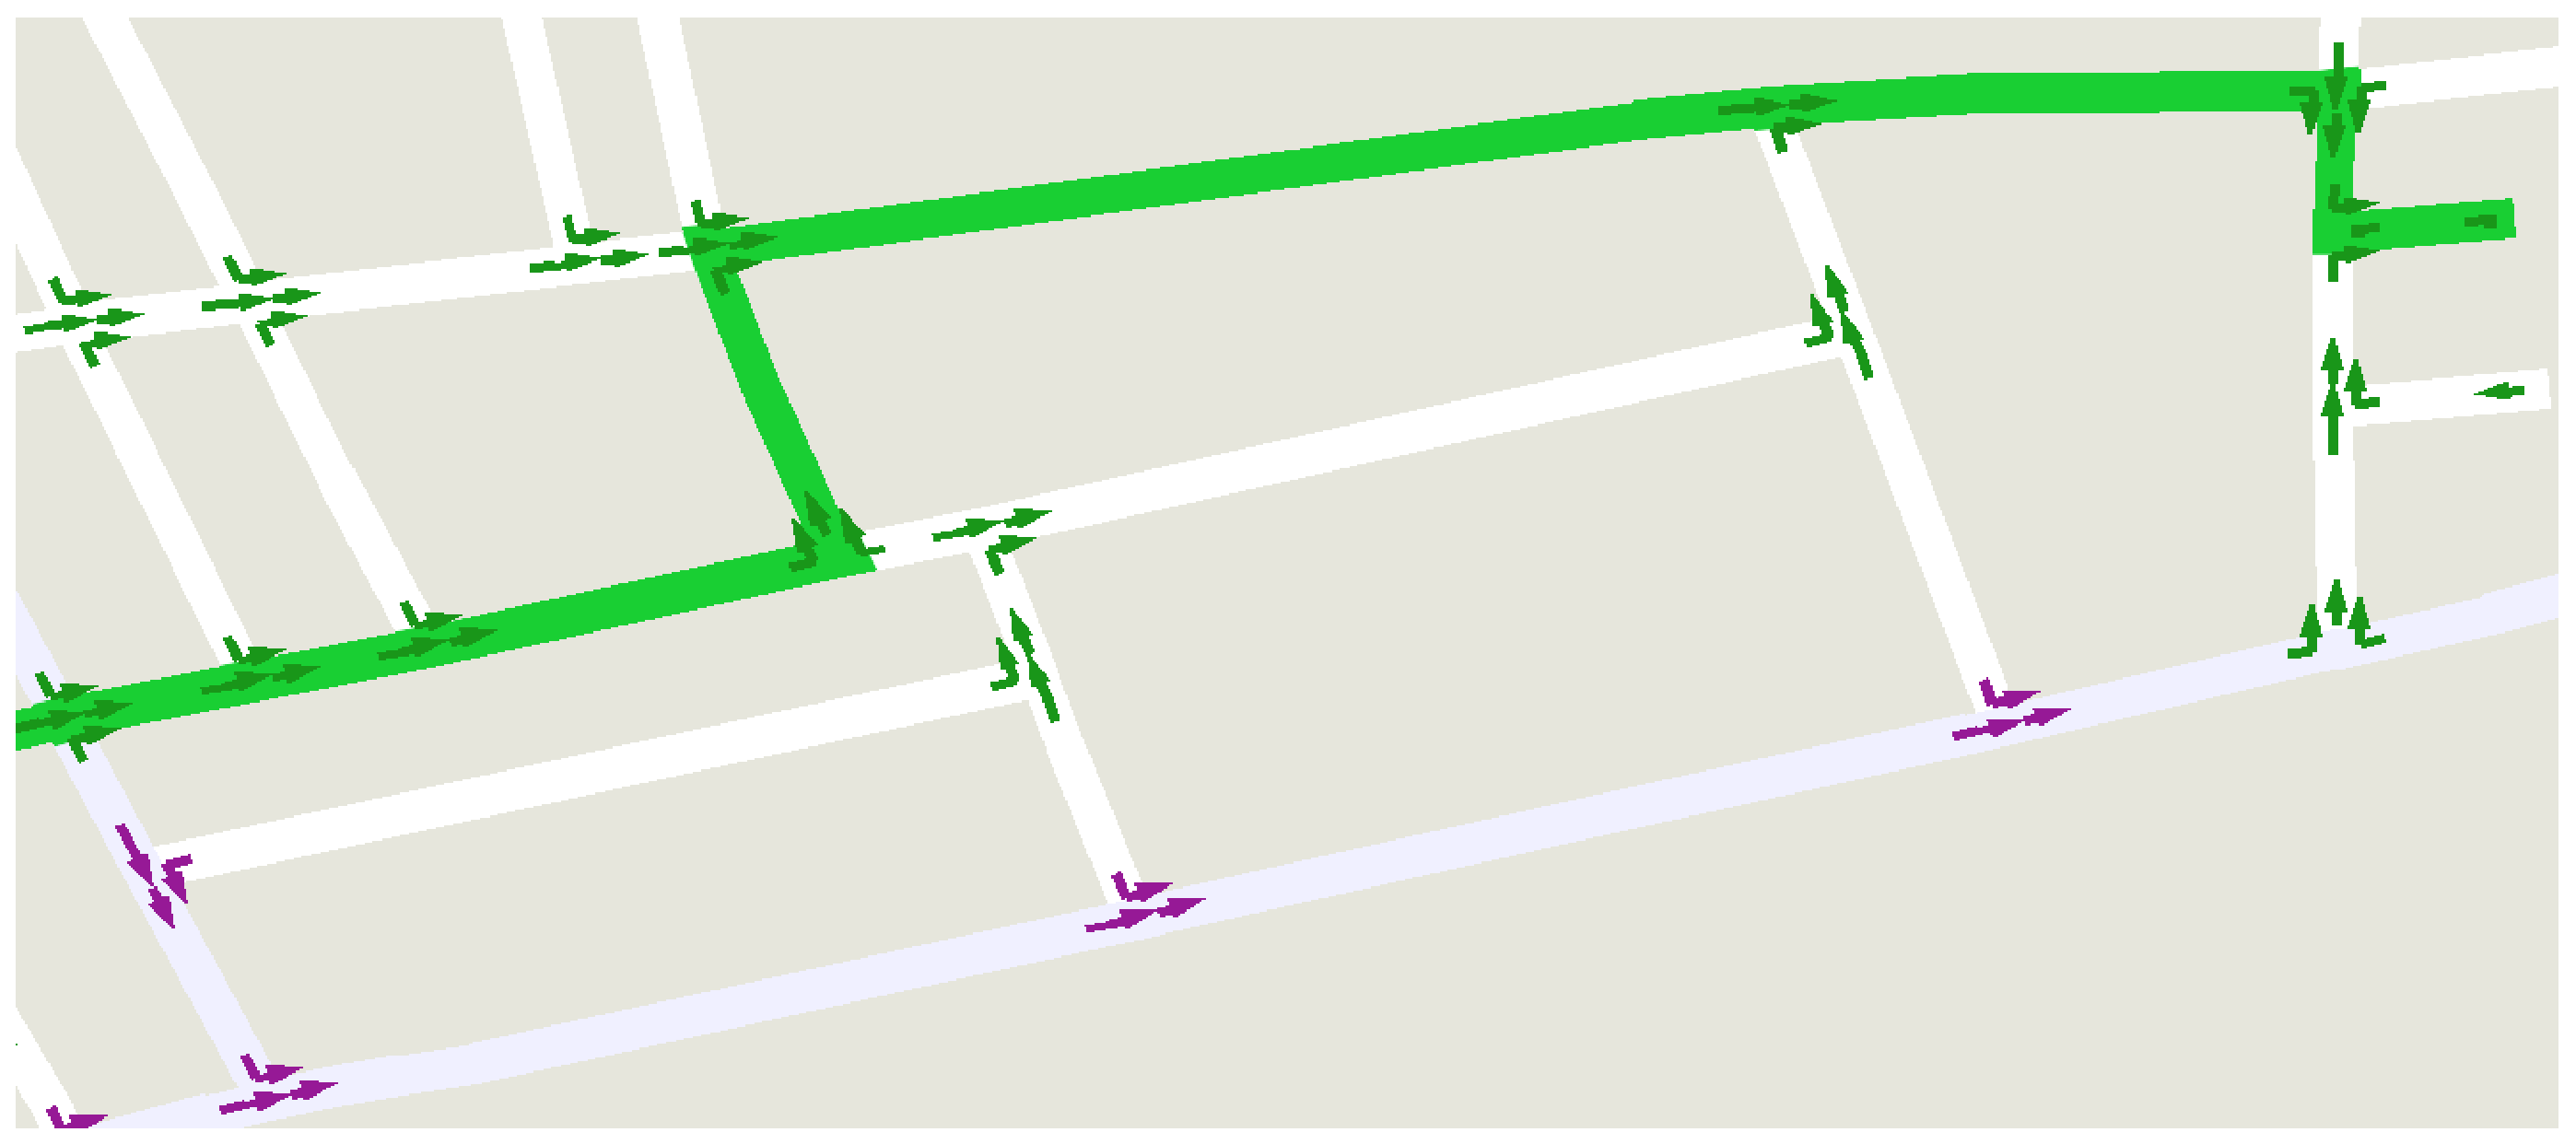
\includegraphics[width=0.75\linewidth]{awake.eps} \\
    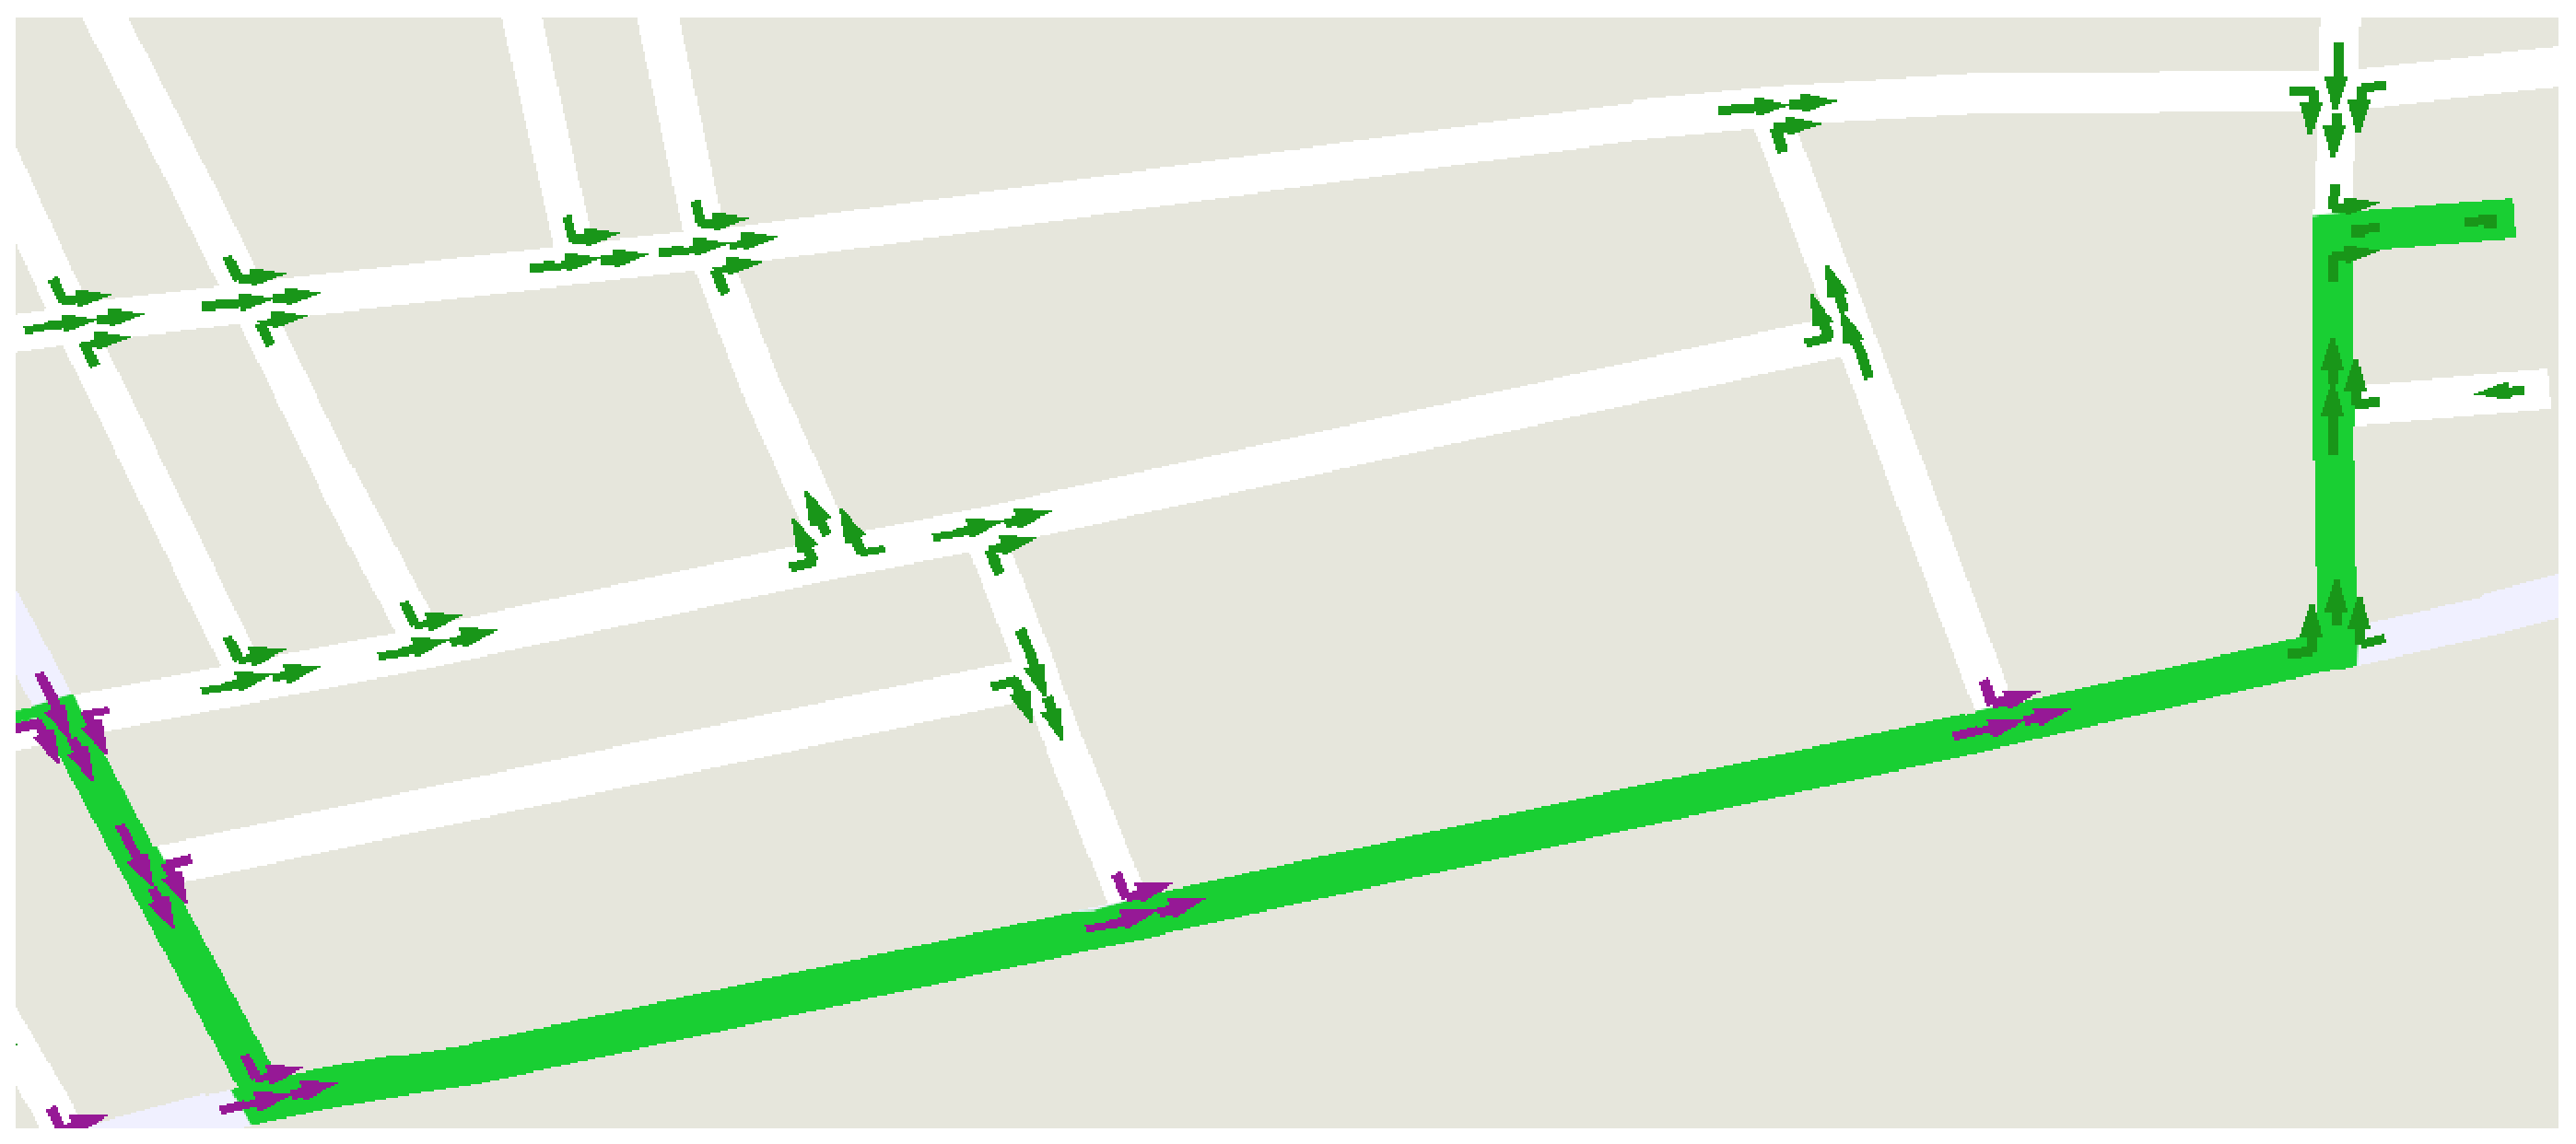
\includegraphics[width=0.75\linewidth]{tired.eps}
    \caption{The policy for awake (above) versus tired (below).}
    \label{fig:example_policy}
\end{center}
\end{figure}


\subsection{GPU Optimized LVI}

We explore the scalability of LVI in a GPU-optimized implementation using CUDA. VI on GPUs has been shown to improve performance and enable scalability~\cite{Johannsson09-GPUBasedMDPSolver,Boussard10-ObservationalPlanningMDPGPU}. Our approach for LVI also exploits the inherent structure of Bellman's optimality equation: independent updates of the values of states. LVI also allows us to run each partition separately, further improving the scalability since it can be distributed among multiple GPU blocks or grids.

Our implementation first transfers the entire LMDP model from the host (CPU) to the device (GPU). Each partition is executed separately, with each Bellman update run in parallel. After convergence, the final policy and values are transferred back from the device to the host. One of the largest performance costs comes from transferring data between host and device, but thankfully LVI can avoid this issue since the model is only read a finite number of times.

\begin{table*}%[htb]
    \small
    \begin{tabular*}{\textwidth}{@{\extracolsep{\fill}} | l | l | l | l | l | l | l |}
        \hline
        City           & $|S|$    & $|A|$    & CPU   & GPU (128)  & GPU (256) & GPU (512) \\
        \hline
        %Amherst        & 496      & 8        & 6075  & 4069       & 4647      & 4669 \\
        Austin         & .     & .       & .   & .      & .      & . \\
        Baltimore      & .     & .       & .   & .      & .      & . \\
        Boston         & 296      & 8        & 2048  & 2259       & 2443      & 2453 \\
        Chicago        & .     & .       & .   & .      & .      & . \\
        Denver         & .     & .       & .   & .      & .      & . \\
        Los Angeles    & .     & .       & .   & .      & .      & . \\
        New York City  & 3608     & 10       & .   & .      & .      & . \\
        Pittsburgh     & .     & .       & .   & .      & .      & . \\
        San Francisco  & .     & .       & .   & .      & .      & . \\
        Seattle        & .     & .       & .   & .      & .      & . \\
        \hline
    \end{tabular*}
    \caption{Summary of timings in milliseconds, varying CPU and GPU (block sizes).}
    \label{tbl:timings}
\end{table*}

Experiments shown in Table~\ref{tbl:timings} were executed with an Intel(R) Core(TM) i7-4702HQ CPU at 2.20GHz, 8GB of RAM, and an Nvidia(R) GeForce GTX 870M graphics card using C++ and CUDA(C) 6.5.

